\section{Seguran\c{c}a de uma CDN} \label{sec:seguranca}
Segundo \cite{ferreira2004novo} seguran\c{c}a \'e definido como um conjunto de a\c{c}\~oes que e dos recursos utilizados para proteger algo ou algu\'em, ou, o que serve para diminuir os riscos ou perigo. Portanto, seguran\c{c}a \'e um tema extramente abrangente e complexo. Podemos falar de t\'opicos como seguran\c{c}a f\'isica, social, de um sistema ou at\'e mesmo de um grupo de servidores interconectados, que \'e o caso da CDN, e ainda coloca-los todos dentro do mesmo grupo. Ou seja, podemos trat\'a-los de forma separada ou analisando o conjunto todo.
 
Ainda dentro de Seguran\c{c}a de CDN podemos tratar de pontos principais, onde o vazamento \'e ponto crucial e mais l\'ogico de ser atacado. 
\begin{figure}[H]
\caption{Objetivos da seguran\c{c}a}
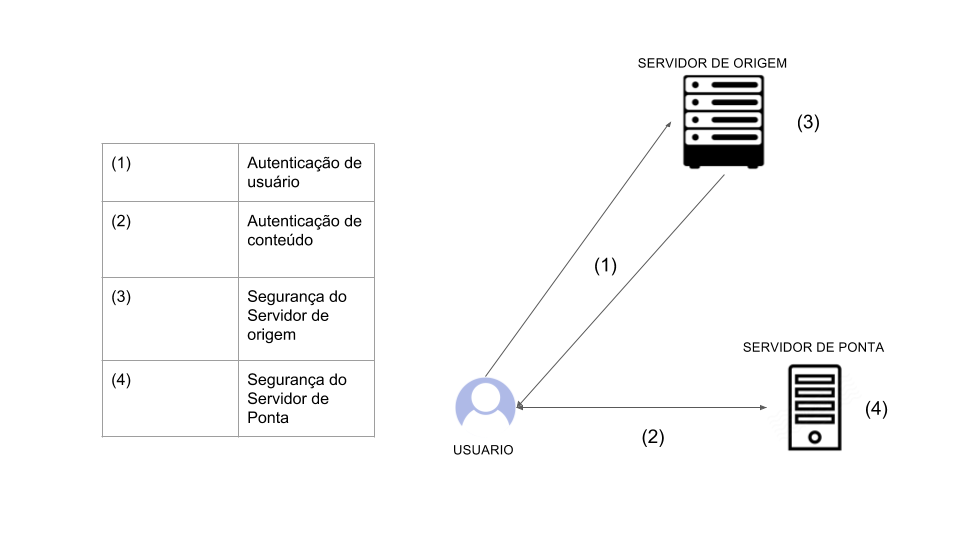
\includegraphics[height=9cm]{Figuras/seguranca_intro.png} 
\label{figura:seguranca_intro}
\end{figure}

Como vemos na figura \ref{figura:seguranca_intro} podemos observar que se tem quatro grandes pontos a serem garantidos em uma rede. Dois deles (1) e (2) de autentica\c{c}\~ao e outros dois (3) e (4) relacionados a integridade. O primeiro trata-se da autentica\c{c}\~ao de usu\'ario que \'e capacidade do sistema de garantir que aquele usu\'ario que est\'a acessando o conte\'udo tem mesmo os requisitos para acess\'a-lo. Ou seja, \'e mesmo um usu\'ario do sistema. Por ser um tema bem abrangente ser\'a tratado com mais profundidade em \ref{subsection:autenticacao_usuario}.

Em segundo lugar temos a autentica\c{c}\~ao de conte\'udo. Que \'e a garantia que o conte\'udo acessado \'e o mesmo buscado pelo usu\'ario, que o usu\'ario tem acesso a ele e tamb\'em \'e um conte\'udo que faz parte da rede de disponibilidade da CDN(que n\~ao \'e um conte\'udo inserido por terceiro sem autoriza\c{c}\~ao pr\'evia). Tudo isso tem que ser minuciosamente tratado e averiguado antes de retornar ao usu\'ario. Tudo isso ser\'a abordado em \ref{subsection:autenticacao_conteudo}.

Nos dois outros, (3) e (4), trata-se da seguran\c{c}a dos servidores. A\'i podemos falar de seguran\c{c}a f\'isica e l\'ogica. Tem-se que levar em conta a forma de acesso de cada um na hora de mensurar os aspectos de seguran\c{c}a de cada um deles. 

No servidor de origem se tem um acesso via HTTP, com um endereço "leg\'ivel". Esse acesso se dar\'a muitas vezes por v\'arias parte do globo, tendo que deix\'a-lo dispon\'ivel , portanto, vulner\'avel \`a diversos tipos de ataque, o que o torna extremamente complexo na hora de definir suas regras de seguran\c{c}a, n\~ao basta apenas subir um \textit{firewall} bloqueando m\'ultiplos acessos, \'e preciso saber exatamente os tipos de aplica\c{c}\~oes que ser\~ao tratadas para assim come\c{c}ar a desenhar as regras de \textit{firewall} que ser\~ao aplicadas.

J\'a no servidor de ponta a preocupa\c{c}\~ao com o acesso via HTTP j\'a \'e uma coisa a menos, visto que muitas vezes o acesso funcionar\'a via redirecionamento do servidor de origem, sendo o controle de endere\c{c}o feito pelo o mesmo. Mas h\'a diversos outros aspectos que tem que serem levados em conta, como parte da autentica\c{c}\~ao de conte\'udo para o usu\'ario, que nada mais \'e que garantir que o usu\'ario para o qual est\'a sendo enviado o conte\'udo tem acesso ao mesmo. Outra grande preocupa\c{c}\~ao \'e quanto a sua disponibilidade, pois \'e necess\'ario que o mesmo esteja "de p\'e" quando for requisitado conte\'udo e que durante o processo de transfer\^encia, caso haja alguma interrup\c{c}\~ao a mesma seja informada ao servidor de origem e o usu\'ario transferido para outro servidor sem que haja muitos danos \`a experi\^encia. Isso sem contar nas enumeras preocupa\c{c}\~oes que se deve ter com servidores. No livro \cite{stallings1995network} se pode aprofundar um pouco mais nessas quest\~oes de seguran\c{c}a na \textit{web}.

Mas para se aprofundar um pouco mais dentro dos conceitos de seguran\c{c}a de usu\'ario e conte\'udo de uma CDN \'e necess\'ario primeiro conhecer um pouco sobre protocolos AAA que ser\'a tratado em \ref{subsection:AAA}.
\subimport{seguranca/}{AAA}
\subimport{seguranca/}{autenticacaousuario}
\subimport{seguranca/}{autenticacaoconteudo}